\documentclass[conference]{IEEEtran}
\IEEEoverridecommandlockouts
% The preceding line is only needed to identify funding in the first footnote. If that is unneeded, please comment it out.
\usepackage{cite}
\usepackage{amsmath,amssymb,amsfonts}
\usepackage{algorithmic}
\usepackage{graphicx}
\usepackage{minted}
\usepackage{textcomp}
\usepackage{xcolor}
\usepackage{polski}
\usepackage{comment}
\usepackage[utf8]{inputenc}
\usepackage{graphicx}
\usepackage{hyperref}
\setlength\parskip{0.5em}

\def\BibTeX{{\rm B\kern-.05em{\sc i\kern-.025em b}\kern-.08em
    T\kern-.1667em\lower.7ex\hbox{E}\kern-.125emX}}
\begin{document}

\title{Gra planszowa ,,Chińczyk'' z systemem AI}

\author{\IEEEauthorblockN{Kacper Burzała}
\IEEEauthorblockA{\textit{nr indeksu: 234943} \\
\textit{Politechnika Wrocławska}\\
Wrocław, Polska \\
}
\and
\IEEEauthorblockN{Przemysław Jedlikowski}
\IEEEauthorblockA{\textit{nr indeksu: 234927} \\
\textit{Politechnika Wrocławska}\\
Wrocław, Polska \\
}
\and
\IEEEauthorblockN{Bartosz Rodziewicz}
\IEEEauthorblockA{\textit{nr indeksu: 226105} \\
\textit{Politechnika Wrocławska}\\
Wrocław, Polska \\
}
}


\maketitle


\section{Streszczenie}
Projekt został zrealizowany w ramach kursu ,,Metody sztucznej inteligencji w projektowaniu gier'', prowadzonego przez dr inż. Wojciecha Kmiecika. Celem projektu jest stworzenie aplikacji pozwalającej na rozegranie gry planszowej ,,Chińczyk'' (znanej także jako ,,Ludo'' oraz ,,Człowieku, nie irytuj się'') na pojedynczym komputerze dla 4 graczy lub zamieniając dowolną ilość graczy na graczy sterowanych komputerem, wykorzystujących propozycję systemu AI. W skład aplikacji umożliwiającej przeprowadzenie rozgrywki we wspomnianej grze wchodzi zarówno logika sterującej grą, jak i graficzny interfejs użytkownika, co umożliwi komfortową rozgrywkę w czasie rzeczywistym. Aplikacja została zaimplementowana w języku GDScript, zaprojektowanym specjalnie na potrzeby silnika Godot \cite{godot}.

\section{Wstępny opis słowny}
Zadaniem aplikacji jest umożliwienie rozegrania partii gry ,,Chińczyk''. W tym celu po jej uruchomieniu na ekranie wyświetla się ekran konfiguracyjny dla typów zawodników (gracz ludzki / gracz komputerowy), a w przypadku gracza sterowanego algorytmem można również określić strategię jego gry. Po przejściu do realnej rozgrywki wyświetlana jest plansza, składająca się z czterdziestu pól, czterech domków oraz czterech schowków. Ponadto na planszy znajduje się 16 pionków, po 4 w każdym z 4 kolorów, reprezentujących poszczególnych graczy oraz kostka do gry. Na ekranie wyświetla się także krótka instrukcja do obsługi programu oraz wskazanie na gracza mającego właśnie kolejkę \cite{wiki}.


Aplikacja umożliwia kolejnym graczom wykonanie swojej kolejki poprzez wykonanie rzutu kostką oraz, w przypadku posiadania legalnego ruchu, wybór pionka, którym zostanie wykonany ruch.  Ponadto program umożliwia przeprowadzenie podstawowych działań składających się na reguły gry takich jak bicie, wprowadzanie pionków do domków, wyprowadzanie pionków ze schowka, ponowienie rzutu po wyrzuceniu ,,szóstki'', czy wykrycie końca rozgrywki w momencie wprowadzenia wszystkich pionków do domku przez jednego z graczy. Dodatkowo aplikacja powinna implementować funkcjonalności usprawniające doświadczenie użytkownika. Jedno z takich funkcjonalności jak menu ustawień umożliwiające dostosowanie ustawień graficznych, zmianę liczby graczy czy zmianę sposobu sterowania. Kolejnymi funkcjami możliwymi do zaimplementowania są obsługa myszy do przesuwania pionków, czy animacja ich przesuwania. Ponadto aplikacja powinna posiadać menu początkowe oraz ekran zakończenia gry wskazujący zwycięzcę.


\section{Słownik pojęć z dziedziny problemu}
Słownik został opracowany na podstawie zasad gry opisanych w \cite{wiki}.
\begin{itemize}
    \item Bicie - Sytuacja, w której pionek jednego koloru wkracza na pole zajmowane przez pionek innego koloru. W takiej sytuacji pionek, który uprzednio zajmował dane pole zostaje ,,zbity'' i powraca do schowka.
    \item Domek - Cztery pola będące docelową lokalizacją pionków danego gracza. Gracz ma prawo wprowadzić pionka do domku dopiero po okrążeniu nim całej planszy, do domku jednego gracza nie mogą wejść pionki innego gracza (koloru). W momencie, w którym jeden z graczy zapełni swój domek wszystkimi swoimi pionkami wygrywa grę.
    \item Gracz - Jedna z czterech osób uczestniczących w grze. Każdy gracz posiada swój unikalny kolor i cztery pionki. Podczas swojej kolejki gracz rzuca kością i decyduje, który pionek zostanie ruszony. W grze uczestniczy czterech graczy.
    \item Kolejka - Moment, w którym dany gracz może wykonać swój ruch. Gracze wykonują swój ruch po kolei, zgodnie ze wskazówkami zegara. Kolejka składa się z rzutu kostką i przesunięcia pionka. W momencie, gdy gracz wyrzucił na kości ,,szóstkę'' powtarza ruch przed zakończeniem kolejki.
    \item Kość - Służy do losowego określenia liczby pól, o które gracz przesunie pionka. Efektem rzutu kością jest liczba oczek z zakresu 1-6.
    \item Kolor - Unikalny identyfikator każdego z graczy określający jego pionki, schowek, pole startowe oraz domek.
    \item Pionek - Figura, którą porusza gracz podczas swojej kolejki w celu przesunięcia jej do domku. Każdy z graczy ma cztery pionki o własnym kolorze i po umieszczeniu wszystkich w domku wygrywa grę.
    \item Plansza - Miejsce rozgrywania gry. Składa się z czterdziestu pól, w tym czterech startowych, czterech domków oraz czterech schowków.
    \item Pole - Część planszy, po której można przesuwać pionki w celu okrążenia planszy i umieszczenia ich w domku. Na planszy znajduje się 36 zwykłych pól oraz 4 pola startowe.
    \item Pole startowe - Cztery pola, na których umieszcza się pionki po wyprowadzeniu ich ze schowka. Każde z pól posiada własny kolor odpowiadający kolorowi gracza posiadającego schowek.
    \item Schowek - Miejsce startowe wszystkich pionków. Celem gracza jest wyprowadzenie tych pionków poprzez wyrzucenie ,,szóstki'' na kości i umieszczenie pionka na odpowiednim polu startowym. Istnieją cztery schowki, po jednym dla każdego gracza.
    \item Ruch - Moment przesunięcia pionka po rzucie kością. Zazwyczaj gracz w jednej kolejce wykonuje jeden ruch, wyjątkiem jest sytuacja, w której gracz wyrzucił ,,szóstkę'' - wtedy po wykonaniu ruchu w nagrodę ponownie rzuca kością i wykonuje dodatkowy ruch przed zakończeniem kolejki.
\end{itemize}


\section{Analiza wymagań użytkownika}
Aplikacja ma za zadanie umożliwienie przeprowadzenia rozgrywki w grę ,,Chińczyk''. W tym celu z punktu widzenia użytkownika aplikacja musi wykonywać dwie czynności: rzut kością do gry oraz wykonanie ruchu wskazanym przez gracza pionkiem o liczbę oczek określoną wykonanym przed ruchem rzutem. Poza tym aplikacja reaguje na dane wejściowe z pierwszej sceny, odpowiednio konfigurując graczy. W ramach każdego wykonywanego ruchu program musi sprawdzić jego legalność i zabronić wykonywania ruchów niedozwolonych, takich jak ruch pionkiem ze schowka w momencie wyrzucenia mniejszej liczby oczek niż 6. W formie graficznej wymagania te obrazuje diagram przypadków użycia.

\begin{figure}[H]
    \centering
    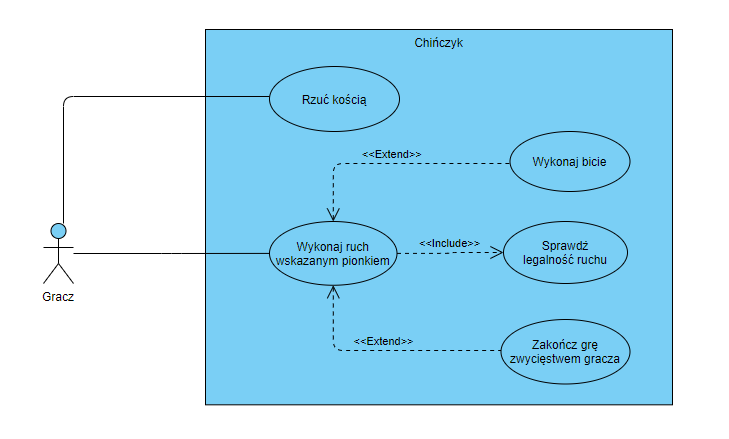
\includegraphics[width=\linewidth]{UseCase.png}
    \caption{Diagram przypadków użycia}
\end{figure}

Aktor w postaci gracza może wykonać dwie podstawowe czynności: rzut kością lub wykonanie ruchu wybranym pionkiem. Integralną częścią wykonywanego ruchu jest sprawdzenie jego legalności, stąd związek zawierania pomiędzy omawianymi przypadkami użycia. W przypadku wykonywania bicia oraz zakończenia gry, te przypadki użycia nie będą występować przy każdym wykonaniu ruch, więc są z nim w związku rozszerzenia.

\section{Modele systemu z różnych perspektyw}
Model systemu zakłada istnienie sześciu klas reprezentujących cztery kluczowe pojęcia ze słownika opisującego dziedzinę oraz dwie klasy pomocnicze. Są to: plansza, kość do gry, gracz, pionek, selektor graczy oraz ustawienia. Taki podział umożliwia reprezentację wszystkich kluczowych pojęć w możliwie najprostszej formie.


Plansza do gry (\texttt(Board)) jest rozbudowaną klasą opisującą i przeprowadzającą rozgrywkę. Zawiera ona wszystkich graczy oraz położenia ich pionków, a także ma dostęp do kości do gry. Ponadto zawiera on zmienne niezbędne do kontrolowania stanu rozgrywki określające stan gry, stan tury, rezultat ostatniego rzutu kostką i wskazującą gracza oczekującego na swoją kolejkę.


Klasa \texttt(Dice) opisująca kość do gry jest prostą klasą przechowującą wygląd kości i umożliwiającą symulowanie jej działania poprzez losowanie liczby z zakresu od 1 do 6 za pomocą funkcji \texttt(rollDice()). Ponadto klasa ta posiada standardową funkcję \texttt(\_ready()) wywoływaną w momencie pojawienia się kości na ekranie po raz pierwszy.


Kolejną klasą jest przedstawiająca gracza klasa \texttt(Player). Każdy gracz reprezentowany jest poprzez \texttt(id), a ponadto przechowuje informacje o własnych pionkach. Do zadań tej klasy należy zainicjowanie pionków za pomocą funkcji \texttt(spawnPawns()) i kontrola ich położenia - funkcja \texttt(isAnyPawnOnBoard()) służy do określenia, czy któryś z czterech pionków wyszedł ze schowka, a funkcja \texttt(areAllPawnsFinished()) sprawdza warunek zwycięstwa, czyli czy wszystkie pionki znajdują się w domku. Dodatkowo klasa ta implementuje wiekszość metod odpowiedzialnych za strategie AI, co czyni ją najbardziej złożoną klasą w grze. W przypadku pracy w bardziej obiektowym języku lepszym rozwiązaniem byłoby zastosowanie polimorfizmu na klasie gracza i rozdzielenie każdej strategii i gracza sterowanego przez człowieka na 4 osobne klasy dziedziczące po jednej klasie wirtualnej.


Następną klasą jest klasa \texttt(PlayerPawn) uosabiająca pionki posiadane przez graczy. Zakłada się, że każdy z pionków ma przypisany do siebie numer \texttt(pawnId) oraz id kontrolującego go gracza (\texttt(playerId)). Ponadto każdy z pionków musi mieć określoną aktualną pozycję (zmienna \texttt(currentPosition)) oraz początkową pozycję (\texttt(startPosition)). Zmienna \texttt(pawnPlace) określa status pionka (w schowku, na planszy, w bazie), a zmienna \texttt(label) przechowuje graficzną reprezentację obiektu. Do określenia pozycji na planszy wykorzystywana jest zmienna \texttt(distanceFromStart), która określa ile pól przebył pionek. Dzięki znajomości całkowitej liczby pól, które pionek musi przebyć przed dotarciem do domku zawsze jesteśmy w stanie precyzyjnie określić jego pozycję na tej trasie. 


Następna klasa (\texttt(PlayerSelection) odpowiada za przygotowanie niezbędnych parametrów wejściowych oraz pełni funkcję ekranu startowego gry. Klasa selektora graczy operuje na tablicy 16-elementowej (4 graczy po 4 ustawienia), a każda zmiana wartości w tej tablicy odpowiada różnym funkcjom modyfikującym obiekty sceny 2D (np. obiekty typu \texttt(Rectangle) lub obiekty typu \texttt(Label), jak również obiekty typu \texttt(Sprite) - tu modyfikacja odbywa się poprzez negowanie cechy widzialności). W propozycjach rozwoju aplikacji pojawił się koncept dostosowywania ustawień graficznych, więc wszystkie zmienne i metody z tym związane powinny zostać dodane do klasy ustawień.


Ostatnia klasa, czyli klasa ustawień to specjalny twór. Z uwagi na ograniczenia Godota i jego operowania na drzewie obiektów zmiana sceny powoduje stworzenie wszystkich obiektów na nowo. Wyjątkiem od tej reguły są specjalne automatycznie ładowane obiekty o nazwie Singleton, których gra tworzy pojedynczą instancję i mogą przechowywać wartości zmiennych pomiędzy scenami. W taki właśnie sposób działa klasa ustawień, która przechowuje parametry dla graczy pomiędzy sceną wyboru ustawień, a sceną faktycznej rozgrywki.


Graficzną reprezentację powyższego opisu stanowi diagram klas:

\begin{figure}[H]
    \centering
    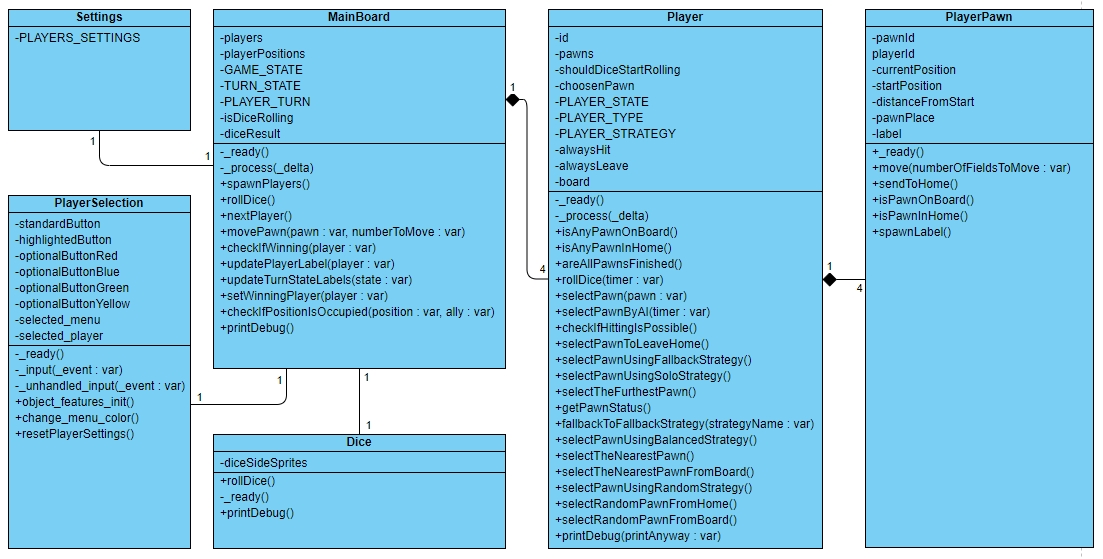
\includegraphics[width=\linewidth]{ClassDiagram.png}
    \caption{Diagram klas}
\end{figure}

Główną klasą kontrolującą stan rozgrywki jest klasa \texttt(MainBoard), w związku z tym posiada ona najwięcej relacji z pozostałymi klasami. Jest ona w stanie komunikować się z klasą \texttt(Dice) dzięki związkowi asocjacji o pojedynczej krotności, a ponadto zawiera w sobie obiekty klasy \texttt(Player). W związku z tym obie klasy łączy związek agregacji całkowitej - obiekt klasy \texttt(MainBoard) zawiera cztery obiekty klasy \texttt(Player). Ponadto w aplikacji istnieje związek agregacji całkowitej pomiędzy klasami \texttt(Player) oraz \texttt(PlayerPawn) - każdy obiekt klasy \texttt(Player) zawiera cztery obiekty klasy \texttt(PlayerPawn)


Główną funkcjonalnością programu jest przeprowadzanie rozgrywki w grę ,,Chińczyk'', dla uproszczenia następne paragrafy opisują zachowanie programu w przypadku wszystkich graczy sterowanych przez ludzi. W tym celu aplikacja musi przyjmować od użytkownika sygnały wejściowe w postaci odpowiednich klawiszy i odpowiednio na nie reagować w zależności od stanu przeprowadzanej rozgrywki. Do monitorowania stanu rozgrywki służą zmienne typu ENUM. Każdy obiekt klasy \texttt(Player) zawiera cztery obiekty klasy \texttt(GAME\_STATE), \texttt(TURN\_STATE) oraz \texttt(PLAYER\_TURN). Pierwsza zmienna odpowiada za ogólny stan rozgrywki, taki jak: gra jeszcze nie rozpoczęta, gra w trakcie, czy gra zakończona. Zmienna \texttt(PLAYER\_TURN) określa zawodnika, którego kolejka właśnie trwa, z kolei zmienna \texttt(TURN\_STATE) reprezentuje moment tury, w którym obecnie znajduje się program i znacząco wpływa na zachowanie danej iteracji pętli głównej.

Na rysunku poniżej przedstawiono diagram sekwencji modelujący pojedynczą iterację pętli głównej odpowiedzialnej za działanie programu.

\begin{figure}[H]
    \centering
    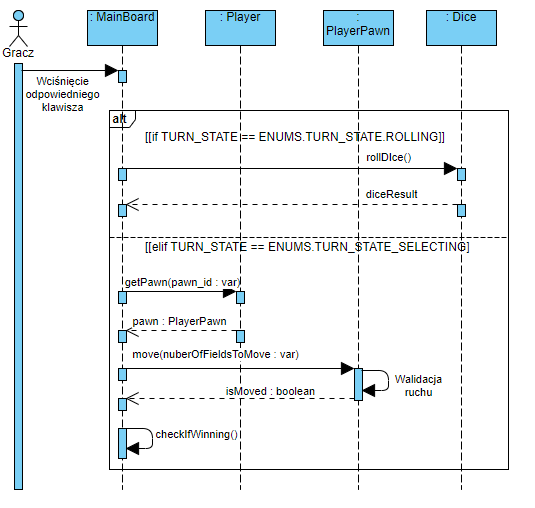
\includegraphics[width=\linewidth]{Sequence.png}
    \caption{Diagram sekwencji modelujący pojedynczą iterację pętli głównej}
\end{figure}

W przypadku gdy stan tury, reprezentowany przez zmienną \texttt(TURN\_STATE) odpowiada wartości \texttt(ENUMS.TURN\_STATE.ROLLING) program jest w fazie poprzedzającej rzut kością. W związku z tym obiekt klasy \texttt(MainBoard) komunikuje się z obiektem klasy \texttt(Dice) poprzez wywołanie funkcji \texttt(rollDice()) zwracającej wynik rzutu kością. Warto wspomnieć, że warunkiem wykonania tej części kodu jest wciśnięcie przez użytkownika klawisza odpowiedzialnego za interakcję, domyślnie jest to spacja. Z kolei jeżeli zmienna \texttt(TURN\_STATE) odpowiada wartości \texttt(ENUMS.TURN\_STATE.SELECTING) program reaguje na klawisze 1-4 odpowiadające poszczególnym pionkom posiadanym przez gracza. Po dokonaniu wyboru obiekt klasy \texttt(MainBoard) rozpoczyna komunikację z odpowiednim obiektem klasy \texttt(Player) w celu otrzymania pionka, który ma zostać przesunięty. Następnie obiekt klasy \texttt(MainBoard) wywołuje funkcję \texttt(move) z argumentem oznaczającym wyrzuconą liczbę oczek, która waliduje żądany ruch i zwraca zmienną binarną określającą, czy ruch jest legalnych i czy zakończył się sukcesem. W takim przypadku następuje sprawdzenie warunku zwycięstwa i zmiana stanu tury.

\section{Graficzny wygląd aplikacji}
Scena PlayerSelection.tscn składa się z 18 pozycji menu, przy czym pierwszy przycisk przenosi do kolejnej sceny (aktywuje grę), 4 kolumny po 4 przyciski do ustawienia playerSettings każdego gracza, a ostatni przyciski powoduje opuszczenie aplikacji.

\begin{figure}[H]
    \centering
    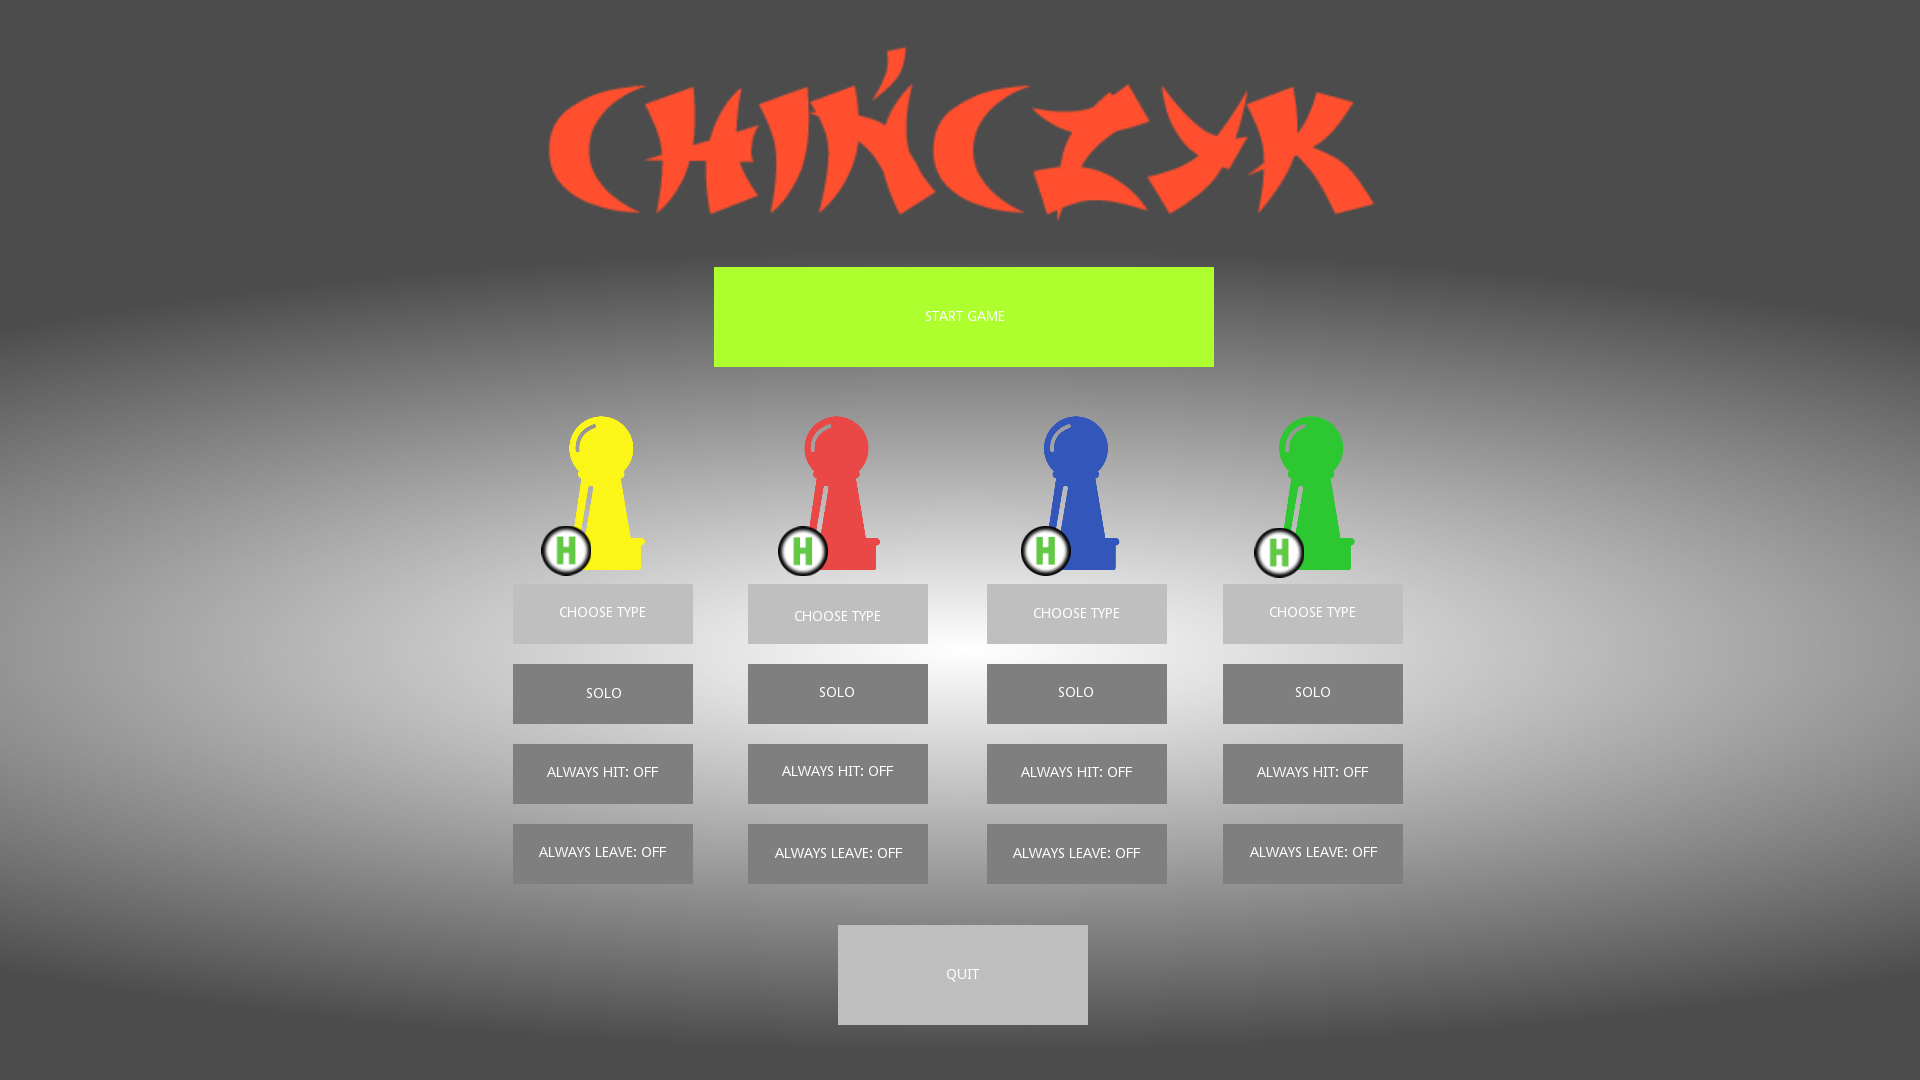
\includegraphics[width=\linewidth]{Scene_1.png}
    \caption{Ekran startowy z ustawieniami gry}
\end{figure}

Scena MainBoard.tscn to realna rozgrywka. Nie ma przycisku, ale za pomoca klawiszcza ESCAPE można wrócić do poprzedniej sceny.

\begin{figure}[H]
    \centering
    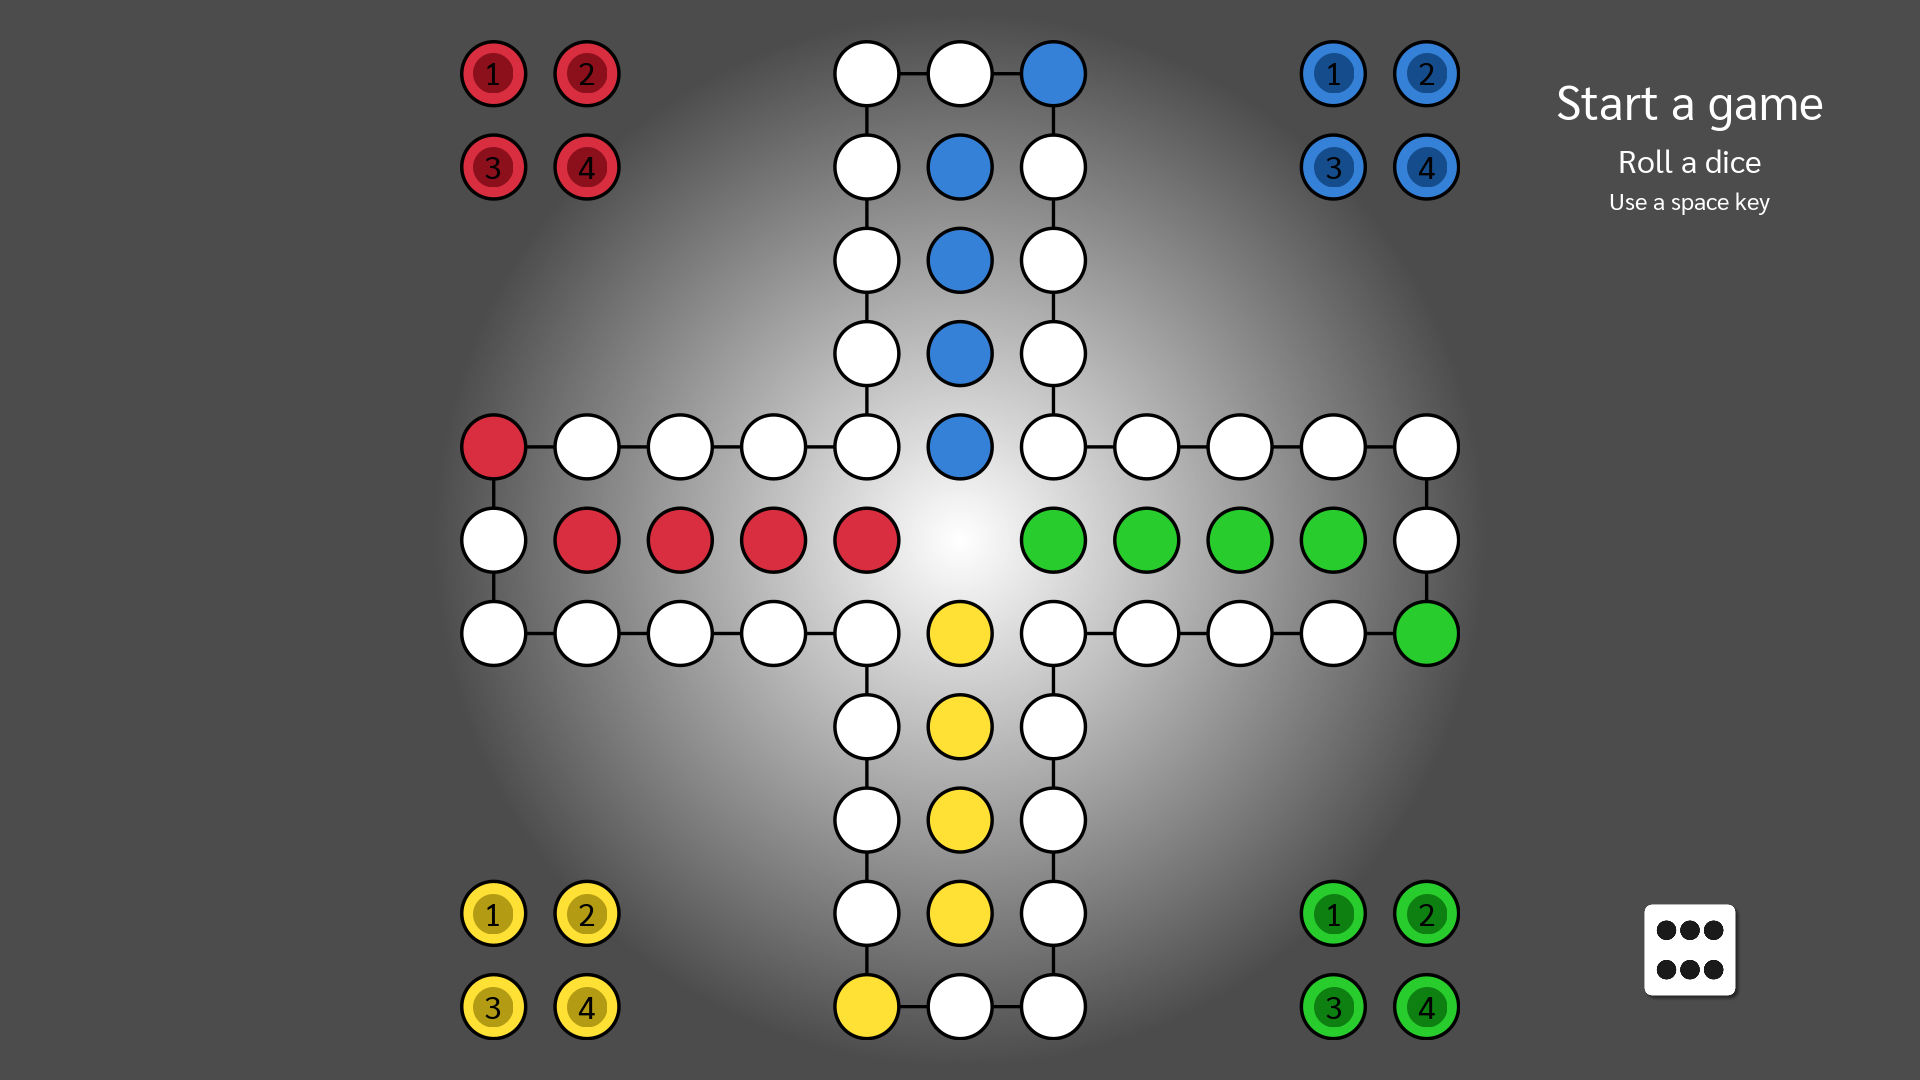
\includegraphics[width=\linewidth]{Scene_2.png}
    \caption{Ekran faktycznej rozgrywki}
\end{figure}

\section{Wprowadzenie systemu AI}
Gracze sterowani za pomocą komputera mogą zostać dostosowani na pierwszej scenie przez odpowiednie przyciski. Pierwsze dwa przyciski odpowiadają za zmianę wartości dwóch zmiennych typu enum: \texttt(ENUMS.PLAYER\_TYPE) (wartości: \texttt(HUMAN), \texttt(AI)) oraz \texttt(ENUMS.STRATEGY) (wartości: \texttt(SOLO), \texttt(BALANCED), \texttt(RANDOM)). Kolejne dwa to proste przyciski boolowe, zmieniające wartości ,,true'' i ,,false'' w zależności od aktualnie ustawionej. Warto nadmienić, że przyciski przekazujące dodatkowy input do programu odnośnie strategii i modyfikacji zachowań graczy komputerowych są podświetlone tylko w przypadku ustawienia wartości ENUMS.PLAYER\_TYPE na AI.


Zaimplementowano 3 wspomnianej wyżej strategie (\texttt(SOLO), \texttt(BALANCED), \texttt(RANDOM)) oraz dwa modyfikatory dodatkowe: \texttt(alwaysHit) (zawsze zbijaj) oraz \texttt(alwaysLeave) (zawsze wychodź). Z punktu konfiguracyjnego taki zestaw przycisków pozwala na 12 kombinacji, lecz z punktu działania algorytmów niektóre kombinacje nawzajem się wykluczają (np. połączenie strategii \texttt(BALANCED) z modyfikacją \texttt(alwaysLeave)).


Pierwsza strategia \texttt(SOLO) oznacza priorytetowe traktowanie jednego pionka w celu jak najszybszego przebycia całej planszy i schowanie go na polu mety. Taka taktyka pozwala maksymalnie uniknąć konfliktów z innymi graczami, a także dostarczać pewny wynik w mniejszych częściach. Pionek, który dojdzie do mety, jest już bezpieczny i nie da się go zbić. W odróżnieniu druga strategia \texttt(BALANCED) polega na zbalansowanym przesuwaniu wszystkich pionków własnej drużyny. Przed ruchem algorytm wykrywa pionka najbliżej ustawionego do punktu startowego danego koloru, po czym przesuwa go o wylosowaną liczbę pól. Równe przesuwanie pionków oznacza większą pulę możliwości zbicia innych graczy, lecz jednocześnie samemu wystawia własne pionki na bycie zbitym. Ostatnia strategia \texttt(RANDOM) losowo wybiera pionki do przesunięcia. Warto nadmienić, że wylosowana szóstka oznacza wyjście pionka z domu z prawdopodobieństwem 50\%. Następnie wybranie konkretnego pionka z domku lub planszy (w zależności od poprzedniego losowania) jest z prawdopodobieństwem $1 / n$, gdzie $n$ to liczba pionków na planszy lub w domku.


Modyfikatory \texttt(alwaysHit) i \texttt(alwaysLeave) współpracują z większością kombinacji ze strategiami. Pierwszy z nich priorytetowo traktuje sytuacje możliwości zbicia innego gracza. Jeśli na planszy żaden inny pionek nie jest w zasięgu zbicia, dodatkowo sprawdza, czy w przypadku wylosowania 6 oczek na pozycji startowej nie znajduje się pionek innego gracza, gdyż zbicie może odbyć się również przy wychodzeniu. Natomiast modyfikator \texttt(alwaysLeave) priorytetowo przeznacza każdą wylosowaną 6-kę oczek na wyciągnięcie wszystkich pionków. W przypadku wyciągania jest to zbliżone do zachowania strategii BALANCED, lecz różnice widoczne byłyby później na planszy.

\section{Kwestie implementacyjne}
Projekt został zaimplementowany na bazie silnika Godot Engine, który jest złożonym, wieloplatformowym narzędziem do tworzenia gier 2D oraz 3D. Umożliwia on w prosty sposób wyeksportować tworzony projekt na najpopularniejsze obecnie systemy operacyjne takie jak Windows, Linux, macOS, Android, iOS, a ponadto na platformy webowe, na przykład HTML. Silnik Godot tworzy kompleksowe środowisko wspierające pełny cykl tworzenia gier, dzięki czemu jest to jedyne narzędzie potrzebne do stworzenia gry ,,Chińczyk''. Godot umożliwia m.in. tworzenie grafiki przy pomocy biblioteki OpenGL ES, wspiera wielokanałowe systemu dźwiękowe a także posiada system ułatwiający tworzenie GUI \cite{godot}.


Wybranym językiem programowania został język GDScrpit, który jest językiem skryptowym zintegrowanym z silnikiem Godot. Umożliwia on tworzenie aplikacji wykorzystujących ten silnik wykorzystując przy tym minimalną możliwą ilość kodu co zwiększa produktywność i ułatwia jego naukę. GDScript jest dynamicznie typowanym językiem upraszczający tworzony kod i nie wymagającym kompilacji do jego testowania \cite{godot}.

\section{Podsumowanie i dyskusja krytyczna}
W ramach tego projektu udało nam się zrealizować i zaimplementować niezbędne funkcjonalności systemu umożliwiającego zagranie w grę ,,Chińczyk'', a także dostarczyć obsługę graczy komputerowych i zapewnić formę sztucznej inteligencji pod postacią różnych strategii. Pomimo, że projekt można by rozszerzyć o pewne dodatkowe funkcjonalności takie jak: menu ustawień graficznych, animację pionków, czy możliwość sterowania myszką, to nie wpłynęłyby one znacząco na zasadnicze zachowanie systemu, a jedynie polepszyły doświadczenie użytkownika, w tym: spełnianie wymogów game loop.


W procesie tworzenia aplikacji zaznajomiliśmy się z tematyką programowania gier, a także poznaliśmy interesujące, otwartoźródłowe środowisko do ich tworzenia - Godot Engine. Implementuje on specjalny język GDScript usprawniający tworzenie gier komputerowych, dzięki czemu po krótkim zapoznaniu się z jego składnią i dokumentacją silnika mogliśmy skupić się na modelu samej aplikacji.

\section*{Kod źródłowy}
Kod źródłowy zaimplementowanej gry jest dostępny w repozytorium pod adresem: \url{https://github.com/baatochan/LudoGame} oraz jako załącznik do tego sprawozdania.

\newpage

\begin{thebibliography}{00}
\bibitem{godot}
Dokumentacja silnika Godot: \url{https://docs.godotengine.org/pl/latest/}

\bibitem{wiki}
Strona na Wikipedii objaśniająca zasady gry ,,Chińczyk'': \url{https://pl.wikipedia.org/wiki/Chińczyk\_(gra\_planszowa)}

\end{thebibliography}


\end{document}